%%%%%%%%%%%%%%%%%%%%%%%%%%%%%%%%%%%%%%%%%
% Programming/Coding Assignment
% LaTeX Template
%
% This template has been downloaded from:
% http://www.latextemplates.com
%
% Original author:
% Ted Pavlic (http://www.tedpavlic.com)
%
% Note:
% The \lipsum[#] commands throughout this template generate dummy text
% to fill the template out. These commands should all be removed when 
% writing assignment content.
%
% This template uses a Perl script as an example snippet of code, most other
% languages are also usable. Configure them in the "CODE INCLUSION 
% CONFIGURATION" section.
%
%%%%%%%%%%%%%%%%%%%%%%%%%%%%%%%%%%%%%%%%%

%----------------------------------------------------------------------------------------
%	PACKAGES AND OTHER DOCUMENT CONFIGURATIONS
%----------------------------------------------------------------------------------------

\documentclass{article}

\usepackage{fancyhdr} % Required for custom headers
\usepackage{lastpage} % Required to determine the last page for the footer
\usepackage{extramarks} % Required for headers and footers
\usepackage[usenames,dvipsnames]{xcolor} % Required for custom colors
\usepackage{graphicx} % Required to insert images
\usepackage{listings} % Required for insertion of code
\usepackage{courier} % Required for the courier font
\usepackage{tikz}
\usepackage{capt-of}
\usepackage{hyperref}
\hypersetup{%
  colorlinks = true,
  linkcolor  = black
}
\usetikzlibrary{automata,positioning}
% Margins
\topmargin=-0.45in
\evensidemargin=0in
\oddsidemargin=0in
\textwidth=6.5in
\textheight=9.0in
\headsep=0.25in

\linespread{1.1} % Line spacing

% Set up the header and footer
\pagestyle{fancy}
\lhead{\hmwkAuthorName} % Top left header
\chead{\hmwkClass: \hmwkTitle} % Top center head
\rhead{\firstxmark} % Top right header
\lfoot{\lastxmark} % Bottom left footer
\cfoot{} % Bottom center footer
\rfoot{Page\ \thepage\ of\ \protect\pageref{LastPage}} % Bottom right footer
\renewcommand\headrulewidth{0.4pt} % Size of the header rule
\renewcommand\footrulewidth{0.4pt} % Size of the footer rule

\setlength\parindent{0pt} % Removes all indentation from paragraphs

%----------------------------------------------------------------------------------------
%	CODE INCLUSION CONFIGURATION
%----------------------------------------------------------------------------------------

\definecolor{MyDarkGreen}{rgb}{0.0,0.4,0.0} % This is the color used for comments
\lstloadlanguages{Python}
\lstset{language=Python,
        frame=single, % Single frame around code
        basicstyle=\small\ttfamily, % Use small true type font
        commentstyle=\usefont{T1}{pcr}{m}{sl}\color{MyDarkGreen}\small, % Comments small dark green courier font
        stringstyle=\color{Purple}, % Strings are purple
        showstringspaces=false, % Don't put marks in string spaces
        tabsize=5, % 5 spaces per tab
        morecomment=[l][\color{Blue}]{...}, % Line continuation (...) like blue comment
        numbers=left, % Line numbers on left
        firstnumber=0, % Line numbers start with line 0
        numberstyle=\tiny\color{Blue}, % Line numbers are blue and small
        stepnumber=1 % Line numbers go in steps of 1
}


% Creates a new command to include a perl script, the first parameter is the filename of the script (without .pl), the second parameter is the caption
\newcommand{\pythonscript}[2]{
\begin{itemize}
\item[]\lstinputlisting[caption=#2,label=#1]{#1.py}
\end{itemize}
}

\def\code#1{\texttt{#1}} % Added by GZZ

%----------------------------------------------------------------------------------------
%	NAME AND CLASS SECTION
%----------------------------------------------------------------------------------------

\newcommand{\hmwkTitle}{CiScal Compiler} % Assignment title
\newcommand{\hmwkDueDate}{Wednesday,\ May\ 24,\ 2017} % Due date
\newcommand{\hmwkClass}{MYY802} % Course/class
\newcommand{\hmwkClassTime}{} % Class/lecture time
\newcommand{\hmwkClassInstructor}{George Manis} % Teacher/lecturer
\newcommand{\hmwkAuthorName}{George Z. Zachos} % Your name

%----------------------------------------------------------------------------------------
%	TITLE PAGE
%----------------------------------------------------------------------------------------

\title{
\vspace{2in}
\textmd{\textbf{\hmwkClass:\ \hmwkTitle}}\\
\normalsize\vspace{0.1in}\small{Due\ on\ \hmwkDueDate}\\
\vspace{0.1in}\large{\textit{\hmwkClassInstructor}}
\vspace{3in}
}

\author{\textbf{\hmwkAuthorName}}
\date{May 24, 2017} % Insert date here if you want it to appear below your name

%----------------------------------------------------------------------------------------

\setcounter{secnumdepth}{3}

\begin{document}

\maketitle

%----------------------------------------------------------------------------------------
%	TABLE OF CONTENTS
%----------------------------------------------------------------------------------------

\newpage
\tableofcontents
\newpage

%----------------------------------------------------------------------------------------
%	Intro
%----------------------------------------------------------------------------------------

\section{About}

\subsection{CiScal language}
CiScal is a minimal programming language that has borrowed many of its characteristics from C and Pascal.
In contrast to its limited capabilities, the development process of a CiScal compiler is quite interesting.

In general, the language does support the following features:
\begin{itemize}
 \item Numeric (integer) constans between -32768 and 32767
 \item \code{if-else}, \code{do-while}, \code{while}, \code{select} and assignment statements
 \item Relational and arithmetic expressions
 \item Definition of functions and procedures; both nested and not
 \item Parameter passing by reference and by value
 \item Recursive function/procedure calls
\end{itemize}

For more information on CiScal capabilities please refer to \code{ciscal-grammar.pdf}

\vspace{0.5cm}
On the other hand, the features below are not supported:
\begin{itemize}
 \item \code{for}-loops
 \item Real numbers
 \item Characters and strings
\end{itemize}


\subsection{CiScal Compiler}
CiScal Compiler (CSC) was developed during the MYY802 - Compilers course at the Department of
Computer Science and Engineering, University of Ioannina. It is written in Python 3 and serves
to transform CiScal source code to Assembly code targeting the MIPS32\footnote{From this point on,
we will refer to MIPS32 as MIPS} architecture. Moreover, transformation of the intermediate code
to ANSI C code is available when possible.

\subsubsection{Using the compiler}
To learn how to use CSC run \verb|./csc.py| and the information below will be printed to console:

\begin{verbatim}
  Usage: ./csc.py [OPTIONS] {-i|--input} INFILE
  Available options:
          -h, --help                Display this information
          -v, --version             Output version information
          -I, --interm              Keep intermediate code (IC) file
          -C, --c-equiv             Keep IC equivalent in C lang file
          --save-temps              Equivalent to -IC option
          -o, --output OUTFILE      Place output in file: OUTFILE
\end{verbatim}

\textbf{Note}: For the course purposes, the \code{--save-temps} option is enabled by default.

\newpage


%----------------------------------------------------------------------------------------
%	Deliverables
%----------------------------------------------------------------------------------------

\section{Deliverables}

\begin{itemize}
 \item 1st Phase (10\%) [Due on March 13, 2017] [Delivered]
 \begin{itemize}
  \item Lexical Analysis
  \item Syntax Analysis
 \end{itemize}

 \item 2nd Phase (30\%) [Due on April 28, 2017] [Delivered]
 \begin{itemize}
  \item Intermediate Code Generation
 \end{itemize}
 
 \item 3rd Phase (10\%) [Due on April 28, 2017] [Delivered]
 \begin{itemize}
  \item Semantic Analysis
  \item Symbol Table
 \end{itemize}

 \item 4th Phase (50\%) [Due on May 24, 2017] [Delivered]
 \begin{itemize}
  \item Final Code Generation (30\%)
  \item Project Report (20\%)
 \end{itemize}
\end{itemize}


%----------------------------------------------------------------------------------------
%	Error Handling
%----------------------------------------------------------------------------------------

\section{Error Handling}

To simplify display of error messages, the following functions have been defined:
\begin{itemize}
 \item \code{perror\_exit()}: Prints an error message to stderr and then program exits
 \item \code{perror()}: Prints an error message to stderr
 \item \code{pwarn()}: Prints a warning to stderr
 \item \code{perror\_line\_exit(ec, lineno, charno, ...)}: Prints line \underline{lineno}
       of the inputfile to stderr with character \underline{charno} highlighted and along
       with and error message. Finally the program exits.
\end{itemize}



\pagebreak

%----------------------------------------------------------------------------------------
%	Lexical Analyzer
%----------------------------------------------------------------------------------------

% To have just one problem per page, simply put a \clearpage after each problem

\section{Lexical Analyzer}

%\subsection{Finite Automata}
The Finite-State Machine (FSM) diagram in Figure \ref{fig:fsm} is a partial graphical representation of the
finite automata implemented in the \code{lex()} function and which is used to convert the input
sequence of characters into a sequence of language tokens. In addition to the states shown below,
there are fourteen (14) more accepting states that correspond to characters: '\code{+}', '\code{-}', '\code{*}', 
'\code{/}', '\code{=}', '\code{,}', '\code{;}', '\code{\{}', '\code{\}}', '\code{(}', '\code{)}', 
'\code{[}', '\code{]}' and '\code{eof}'. Transition to these states is triggered only from initial state $s_0$.
\vspace{1cm}

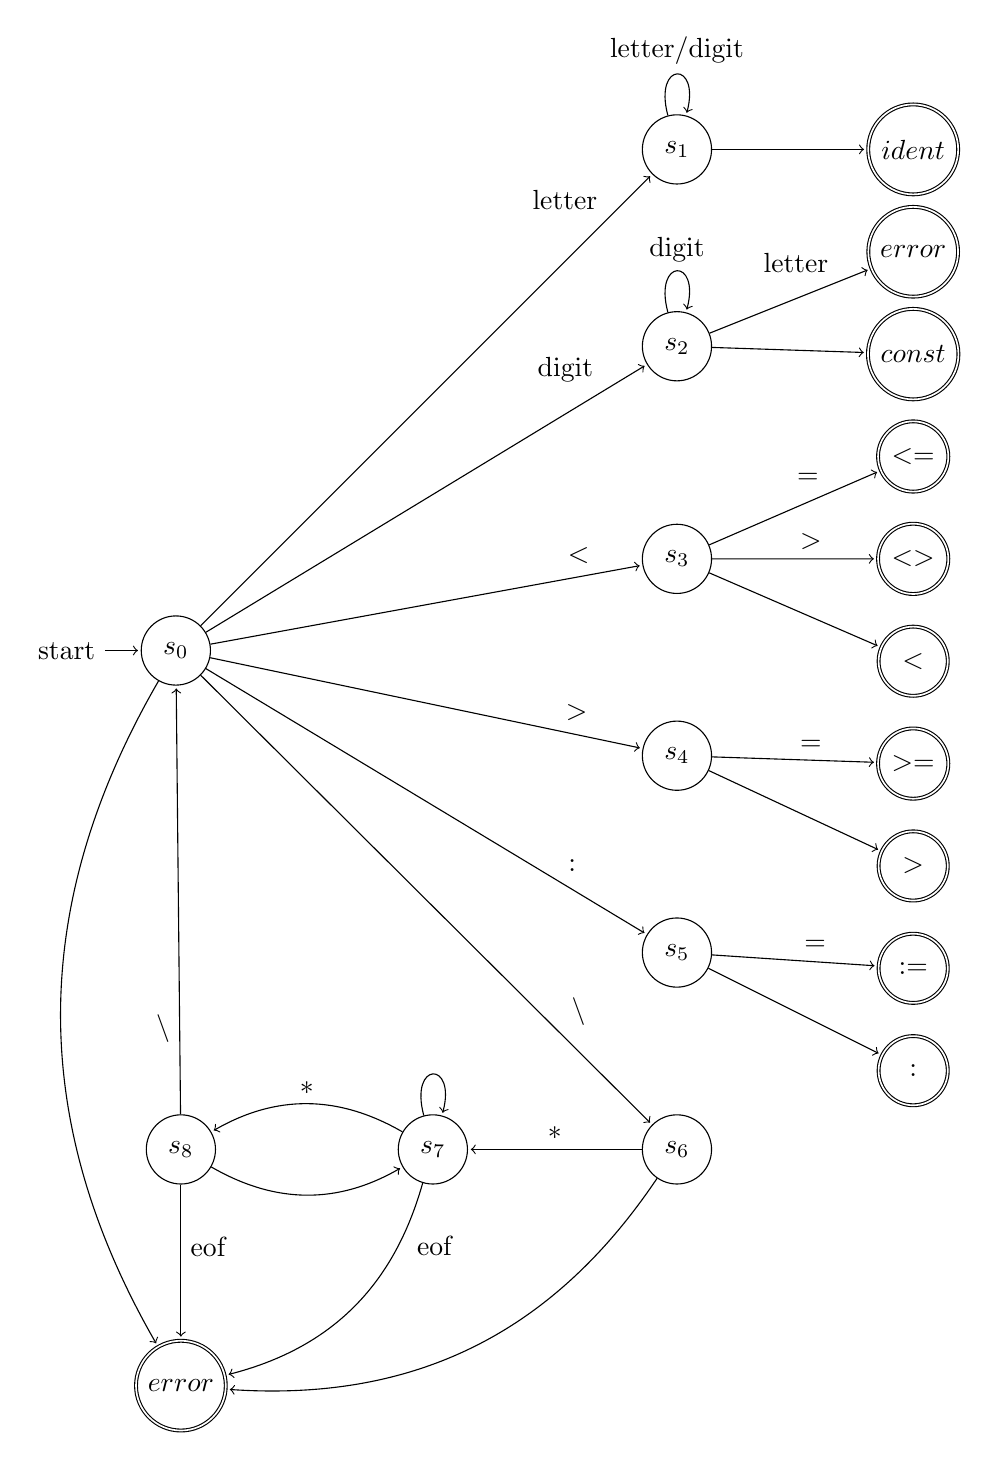
\begin{tikzpicture}[shorten >=1pt,node distance=3cm,on grid,auto]
  \tikzstyle{every state}=[align=center]
  \node[state,initial] (s_0)   {$s_0$};
  \node[state] (s_1) [above right=9cm of s_0] {$s_1$};
  \node[state, accepting] (ident) [right=of s_1] {$ident$};
  \node[state] (s_2) [below=2.5cm of s_1] {$s_2$};
  \node[state, accepting] (err_0) [below =1.3cm of ident] {$error$};
  \node[state, accepting] (const) [below =1.3cm of err_0] {$const$};
  \node[state] (s_3) [below=2.7cm of s_2] {$s_3$};
  \node[state, accepting] (leq) [below =1.3cm of const] {$<=$};
  \node[state, accepting] (neq) [below =1.3cm of leq] {$<>$};
  \node[state, accepting] (lss) [below =1.3cm of neq] {$<$};
  \node[state] (s_4) [below=2.5cm of s_3] {$s_4$};
  \node[state, accepting] (geq) [below =1.3cm of lss] {$>=$};
  \node[state, accepting] (gtr) [below =1.3cm of geq] {$>$};
  \node[state] (s_5) [below=2.5cm of s_4] {$s_5$};
  \node[state, accepting] (become) [below =1.3cm of gtr] {$:=$};
  \node[state, accepting] (colon) [below =1.3cm of become] {$:$};
  \node[state] (s_6) [below=2.5cm of s_5] {$s_6$};
  \node[state] (s_7) [left=3.1cm of s_6] {$s_7$};
  \node[state] (s_8) [left=3.2cm of s_7] {$s_8$};
  \node[state, accepting] (err_1) [below=3cm of s_8] {$error$};
    \path[->] 
    (s_0) edge node [pos = 0.9] {letter} (s_1)
          edge node [pos = 0.9] {digit} (s_2)
          edge node [pos = 0.9] {$<$} (s_3)
          edge node [pos = 0.8] {$>$} (s_4)
          edge node [pos = 0.8] {$:$} (s_5)
          edge node [pos = 0.8] {$\backslash$} (s_6)
          edge [bend right] node {} (err_1)
    (s_1) edge [loop above] node {letter/digit} (s_1)
          edge node {} (ident)
    (s_2) edge [loop above] node {digit} (s_2)
          edge node [pos= 0.5, below] {} (const)
          edge node [pos= 0.8] {letter} (err_0)
    (s_3) edge node [pos = 0.7] {$=$} (leq)
          edge node [pos = 0.6] {$>$} (neq)
          edge node {} (lss)
    (s_4) edge node [pos = 0.6] {$=$} (geq)
          edge node {} (gtr)
    (s_5) edge node [pos = 0.5] {$=$} (become)
          edge node {} (colon)
    (s_6) edge node [above] {$*$} (s_7)
          edge [bend left] node {} (err_1)
    (s_7) edge [loop above] node {} (s_7)
          edge [bend right] node [above] {$*$} (s_8)
          edge [bend left] node [pos = 0.15] {eof} (err_1)
    (s_8) edge node [pos = 0.2] {$\backslash$} (s_0)
          edge [bend right] node {} (s_7)
          edge node [pos = 0.4, right] {eof} (err_1);
\end{tikzpicture}
\captionof{figure}{Partial FSM diagram of lexical analyzer's finite automata}\label{fig:fsm}

\pagebreak

\subsection{Implementation Details}

\subsubsection{Custom Classes}
During the implementation of the lexical analyzer, a couple of classes were defined.
The first class defined was the \code{TokenType} class which is an enumeration that maps token
types to enumerated constants. The other class was the \code{Token} class and was defined to group
all useful information related to a token and that should be available to the syntax analyzer. 
This information includes:
\begin{itemize}
 \item \code{tktype}: token type (attribute of the \code{TokeType} enumeration)
 \item \code{tkval}: the actual token value
 \item \code{tkl}: the line number of the input file that the token was found
 \item \code{tkc}: the offset of the token's first character from the start of line \code{tkl}
\end{itemize}

% \pythonscript{token-class}{Token Class}

\subsubsection{Data Structures}
The \code{token} dictionary maps actual keyword values to the corresponding \code{TokenType} 
attributes and serves code simplicity.
\pythonscript{token-dict}{Token type/value dictionary}

\subsubsection{Return Value}
The \code{lex()} function returns an object of type \code{Token} to the syntax analyzer.

%----------------------------------------------------------------------------------------
%	Syntax Analyzer
%----------------------------------------------------------------------------------------

\section{Syntax Analyzer}

In order for the syntax analysis to take place, a function for each grammar rule was defined. 
In the \code{parser()} function, the global variable \code{token} is assigned the
\code{Token} class instance returned by the first call to \code{lex()}. Then the \code{program()}
function that implements the \code{<PROGRAM>} grammar rule is called and upon success, a last
check takes place to ensure that \code{EOF} follows program end. All functions implementing
grammar rules expect \code{token} to be ready for ``consumption'' and as a consequence 
replace it if needed.

\section{Implementation Specifics}
\subsection{Handling of numeric constants}
CiScal source code files can contain (integer) numeric constants between -32768 and 32767 and
an optional sign (\code{+} or \code{-}) may precede the constant. In case an illegal constant
value is found, an error message should be printed to console. Performing that
check is a bit tricky for the following reasons:
\begin{itemize}
 \item It cannot take place during lexical analysis - This happens because \code{+} and \code{-}
       are terminal symbols and as soon as they are identified, should be returned to the syntax
       analyzer. Moreover, during lexical analysis there is no way to tell if \code{+} and \code{-}
       is a sign or an operator (to put it better, if it is a unary or a binary operator).
       Nevertheless, if the range $[-32768, 32767]$ was symmetrical, the check would be sign
       independent and could take place in the \code{lex()} function.
 \item The syntax analyzer expects from \code{lex()} to return a signed number - This is because
       of CiScal's grammar rules and specifically rule \code{<TERM> ::= <FACTOR> (<MUL\_OPER> <FACTOR>)*}
       when \code{<FACTOR> ::= CONSTANT}. According to these rules, expressions like \code{-2 * -3}
       will trigger a syntax error. In this example, after the multiplication operator the syntax
       analyzer expects a numeric constant but the subtraction operator will be encountered.
\end{itemize}

For theses reasons, syntax rule \code{<FACTOR> ::= CONSTANT | (<EXPRESSION>) | ID <IDTAIL>} was
changed to \code{<FACTOR> ::= <OPTIONAL\_SIGN> CONSTANT | (<EXPRESSION>) | ID <IDTAIL>}.

\textbf{Important}: This change has no impact in the manipulation of numeric constants in the \code{<SELECT-STAT>}
rule and consequently an optional sign preceding a case constant is illegal.

\subsection{Exit Statement}
The \code{exit} statement is supported in nested do-while loops. When it is encountered, the currently
executing loop is immediately terminated and the program control resumes at the next statement following
the loop.

\newpage

%----------------------------------------------------------------------------------------
%	Intermediate Code Generation
%----------------------------------------------------------------------------------------

\section{Intermediate Code Generation}
Intermediate code, also known as intermediate representation is a code used internally by the compiler
in order to represent source code. This code is then used to generate assembly instructions that will finally
be converted to executable machine code. This intermediate representation is machine independent
and is designed to be conducive for further processing, such as optimization\footnote{CiSal Compiler
does not perform any optimazations.} and translation. The intermediate representation used in the CiScal
Compiler is known as \textbf{three-address code}. The name derives because its instructions consist of
at most three\footnote{Instructions with fewer operands may occur.} operands. The combination of three
operands and one operator constitute a \textbf{quadruple} to which we will refer to as a quad. Each quad
can be referenced using a label (non-negative integer). In addition to the three-address code generation,
CSC supports generation of intermediate code equivalent in ANSI C and the generated code is ready to compile
using the underlying system's C compiler. The transformation to ANSI C code takes place only when nested
function definitions do not exist in user program, as it is not supported by the language specifications.
On a later version of CSC, we plan to support nested functions using a GNU C extension provided by the GNU
C Compiler\footnote{\url{https://www.gnu.org/software/gnu-c-manual/gnu-c-manual.html\#Nested-Functions}}.


\subsection{Implementation Details}

\subsubsection{Custom Classes}
While implementing intermediate code generation, the \code{Quad} class was defined which
serves to hold the information of a quadruple. This information is the following:
\begin{itemize}
 \item \code{label}: the label to reference the quad.
 \item \code{op}: the operator to be applied to the source operands.
 \item \code{arg1}: operand \#1, 1st source.
 \item \code{arg2}: operand \#2, 2nd source.
 \item \code{res}: operand \#3, destination.
\end{itemize}

\subsubsection{Global Data}
The following global variables and data structures were used:
\begin{itemize}
 \item \code{nextlabel}: Holds the label (non-negative integer) which will be used to reference
                         the next \code{Quad} to be generated.
 \item \code{next\_tmpvar}: Used to implement the naming convention of temporary variables.
                            (Temporary variable format: T\_$<$next\_tmpvar$>$).
 \item \code{tmpvars}: A dictionary holding temporary variable names.
 \item \code{quad\_code}: A list that holds the \code{Quad} objects generated while parsing
                          the source code of the user program.
\end{itemize}

\newpage

\subsubsection{Function Definitions}
The following functions were defined while implementing the intermediate code generation:
\begin{itemize}
 \item \code{next\_quad()}: Returns the label of the next quad to be generated.
 \item \code{gen\_quad(op, arg1, arg2, res)}: Generates a new quad and appends it to the current quad list
                                              representing input source code.
 \item \code{new\_temp()}: Creates a new temporary variable named \code{T\_n}, with $n>=0$ and returns its name.
 \item \code{empty\_list()}: Creates a new (empty) list that will be used to hold quad labels
                             and returns a reference to it.
 \item \code{make\_list(label)}: Has the same effect of \code{empty\_list()} but also adds \code{label} to the
                                 newely created list.
 \item \code{merge(list1, list2)}: Merges two lists holding quad labels.
 \item \code{backpatch(list, res)}: Replaces the \code{res} attribute\footnote{Destination/3rd operand.} 
                                    of all the quadruples referenced by the labels in \code{list}.
 \item \code{generate\_int\_code\_file()}: Generates the file containing the intermediate code of the user program.
\end{itemize}


For the transformation of the three-address code to ANSI C equivalent code, the following functions
were further defined:
\begin{itemize}
 \item \code{transform\_to\_c(quad)}: Transforms a quad to ANSI C code.
 \item \code{find\_var\_decl(quad)}: A naive way to find which variables are used as operands, starting from
                                     quad \code{quad} and until the end of the block. It returns a list with all
                                     the variable identifiers encountered. This will help during variable declaration.
 \item \code{transform\_decls(vars)}: Given a list of variable identifiers, returns a string with a valid C
                                      variable declaration.
 \item \code{generate\_c\_code\_file()}: Generates the file containing the ANSI C equivalent code of the
                                         intermediate code.
\end{itemize}

\newpage

%----------------------------------------------------------------------------------------
% Symbol Table
%----------------------------------------------------------------------------------------

\section{Symbol Table}
The symbol table is a data structure used by the compiler, where each identifier (a.k.a. symbol) in a program's
source code is associated with information relating to its declaration or appearance in the source.


\subsection{Implementation Details}

\subsubsection{Custom Classes}
Implementing the symbol table, included definition of the following classes containing the corresponding attributes:

\begin{itemize}
 \item \code{Scope}
    \begin{itemize}
    \item \code{nested\_level}: Nested level of scope.
    \item \code{enclosing\_scope}: Reference to a \code{Scope} object.
    \item \code{entities}: List containing all the entities of the scope. New entities
                           are appended at the tail of the list.
    \item \code{tmp\_offset}: Holds the current offset that results after taking into account all parameters,
                              variables (temporary and explicit). It will later be used to update a function's framelength.
    \end{itemize}
  \item \code{Argument}
    \begin{itemize}
    \item \code{par\_mode}: How the argument to the function is passed ("CV" or "REF").
    \item \code{next\_arg}: Reference to the following \code{Argument} object.
    \end{itemize}
  \item \code{Entity}
    \begin{itemize}
    \item \code{name}: Entity name (identifier returned by lexical analyzer).
    \item \code{etype}: Entity type ("VARIABLE", "FUNCTION","PARAMETER","TMPVAR").
    \end{itemize}
  \item \code{Variable} [Extends \code{Entity} Class]
    \begin{itemize}
    \item \code{offset}: Offset of variable with regard to frame start.
    \end{itemize}
  \item \code{Function} [Extends \code{Entity} Class]
    \begin{itemize}
    \item \code{ret\_type}: "int" for CiScal functions or "void" for procedures.
    \item \code{start\_quad}: Quad label of the first quad of the function.
    \item \code{args}: A list containing all function arguments (\code{Argument} objects).
    \item \code{framelength}: The function's framelength.
    \end{itemize}
  \item \code{Parameter} [Extends \code{Entity} Class]
    \begin{itemize}
    \item \code{par\_mode}: "in" and "inout" for \code{TokenType.INSYM} and \code{TokenType.INOUTSYM} respectively.
    \item \code{offset}: Offset of parameter with regard to frame start.
    \end{itemize}
  \item \code{TmpVar} [Extends \code{Entity} Class]
    \begin{itemize}
    \item \code{offset}: Offset of (temporary) variable with regard to frame start.
    \end{itemize}
\end{itemize}

\subsubsection{Global Data}
The following global variables and data structures were used:
\begin{itemize}
 \item \code{scopes}: A list holding \code{Scope} objects. Each new scope is appended at the end of the list.
\end{itemize}

\subsubsection{Function Definitions}
The following functions were defined while implementing the symbol table:
\begin{itemize}
 \item \code{add\_new\_scope()}: Add a new scope.
 \item \code{print\_scopes()}: Print current scope and its enclosing ones.
 \item \code{add\_func\_entity(name)}: Add a new function entity.
 \item \code{update\_func\_entity\_quad(name)}: Update the start quad label of a function entity.
 \item \code{update\_func\_entity\_framelen(name, framelength)}: Update the framelength of a function entity.
 \item \code{add\_param\_entity(name, par\_mode)}: Add a new parameter entity.
 \item \code{add\_var\_entity(name)}: Add a new variable entity.
 \item \code{add\_func\_arg(func\_name, par\_mode)}: Add a new function argument to a given function.
 \item \code{search\_entity(name, etype)}: Search for an entity named \code{name} of type \code{etype}.
 \item \code{search\_entity\_by\_name(name)}: Search for an entity named \code{name}.
 \item \code{unique\_entity(name, etype, nested\_level)}: Check if entity named \code{name} of type \code{etype}
                                                        at nested level \code{nested\_level} is redefined.
 \item \code{var\_is\_param(name, nested\_level)}: Check if a variable entity named \code{name} already 
                                                   exists as a parameter entity at nested level \code{nested\_level}.
\end{itemize}

\newpage

%----------------------------------------------------------------------------------------
% Final Code
%----------------------------------------------------------------------------------------

\section{Final Code}
The final code produced by the CiScal Compiler targets the MIPS\footnote{\url{https://en.wikibooks.org/wiki/MIPS_Assembly/MIPS_Architecture}} architecture and
is ready to assemble using MARS 4.5 (MIPS Assembler and Runtime 
Simulator)\footnote{\url{http://courses.missouristate.edu/KenVollmar/mars/}}.

\subsection{Implementation Details}

\subsubsection{Global Data}
The following global variables and data structures were used:
\begin{itemize}
 \item \code{actual\_pars}: A list holding \code{Quad} objects corresponding to subprogram parameters
                            as discovered while traversing intermediate code. It is then used to validate
                            parameter passing.
\end{itemize}

\subsubsection{Function Definitions}
The following functions were defined while implementing the symbol table:
\begin{itemize}
 \item \code{gnvlcode(v)}: Load in register \code{\$t0} the address of the non-local variable \code{v}.
 \item \code{loadvr(v, r)}: Load immediate or data \code{v} from memory to register \code{\$t\{r\}} (e.g. \code{\$t2}).
 \item \code{storerv(r, v)}: Store the contents of register \code{\$t\{r\}} to the memory allocated
                             for variable \code{v}.
 \item \code{gen\_mips\_asm(quad, block\_name)}: Generate the assembly code for quad \code{quad}.
                                              \code{block\_name} is the name of the block that is
                                              currently translated into final code.
 \item \code{check\_subprog\_args(name)}: Check if actual parameters of subprogram \code{name}
                                          are of the same type as typical parameters.
                                          
\end{itemize}

\subsection{Implementation Specifics}
During the stage of the final code generation, a number of changes have taken
place\footnote{Without regard to a possible conflict with the handout.}.

These are the following:
\begin{itemize}
 \item A number of assembler directives were added across the output file as shown below:
  \begin{lstlisting}
  .globl L_x   # Declare that symbol L_x is global and can be
               # referenced from other files. L_x is a text tag
               # (label) pointing at the start of the main program.
  .text        # The next items are put in the user text segment.
  # ...
  # Assembly code produced while translating intermediate code...
  # ...
  .data        # The following data items should be stored in
               # the data segment.
  newline: .ascizz "\n"   # Store the string "\n" in memory and
                          # null-terminate it. Use label 'newline'
                          # to reference it.
  \end{lstlisting}
  \newpage
 \item Instruction \code{add} (R format\footnote{\url{https://en.wikibooks.org/wiki/MIPS_Assembly/Instruction_Formats\#R_Format}})
       was replaced by \code{addi} (I format\footnote{\url{https://en.wikibooks.org/wiki/MIPS_Assembly/Instruction_Formats\#I_Format}})
       in all cases that immediates were used.
 \item Memory access related instructions (\code{lw}, \code{sw})\footnote{\code{lw} and \code{sw} are of I format}
       were modified to be of the following format:\\ \verb|OP $rt, offset($rs)|, even when offset equals zero
       and can be omitted (e.g. \verb|OP $rt, 0($rs)|).
 \item The final code produced by an \code{out} quad (\verb|out, x, _, _|) is the following:
   \begin{lstlisting}
   li $v0, 1   # service code 1: print the integer stored in $a0
   li $a0, x   # load desired value into argument register $a0
   syscall     # perform the service specified in $v0
  \end{lstlisting}
       Nevertheless, \code{x} can be either a variable identifier or a numeric constant (immediate).
       In case of it being a variable name, instruction \code{li \$a0, x} will fail to assemble.
       To fix this problem the produced code was modified to match:
  \begin{lstlisting}
   # code generated by loadvr(x, '9')
   li $v0, 1
   add $a0, $t9, $zero  # move register content from $t9 to $a0
   syscall
  \end{lstlisting}
 \item For a more aesthetic result regarding the output of the print statement, three more instructions
       were added to the produced code of an \code{out} quad in order for a newline character to be printed
       after every integer print. The lines added are:
  \begin{lstlisting}
  la $a0, newline  # load the addr. of the string pointed by label 'newline'
  li $v0, 4        # service code 4: print the null terminated string at Mem[$a0]
  syscall
  \end{lstlisting}
 \item In MIPS architecture, stack grows from larger to smaller memory
       addresses\footnote{\url{https://www.cs.umd.edu/class/sum2003/cmsc311/Notes/Mips/stack.html}}.
       Because MIPS does not provide an explicit push and pop instruction for manipulating the stack,
       modifying the stack pointer (\verb|$sp| or \verb|$29|) directly is required. Pushing to stack
       and poping from stack requires decreasing and increasing the value of \verb|$sp| respectively.
       For this reason, instructions manipulating the value of stack and frame pointer were changed
       to follow this specification.
 \item The final code produced by a \code{retv} quad was modified to actually return
       program control to the caller and not only to access its frame and update the return value.
       This was done by adding:
  \begin{lstlisting}
   lw $ra, 0($sp)   # Restore the value of $ra. In case of leaf procedures
                    # it is not actually required.
   jr $ra           # jump to the return address
  \end{lstlisting}
 \item Finally, the \code{halt} quad results in the following assembly code:
 \begin{lstlisting}
   li $v0, 10   # service code 10: exit (terminate execution)
   syscall
  \end{lstlisting}
\end{itemize}

\end{document}